\documentclass[border=8pt]{standalone}
\usepackage{tikz-cd}
\usepackage{amsmath,amssymb}
\usepackage{pgfplots}
\pgfplotsset{compat=1.18}
\definecolor{cubicgold}{RGB}{203,157,69}
\definecolor{lineA}{RGB}{157,39,54}
\definecolor{lineB}{RGB}{41,103,161}
\definecolor{lineC}{RGB}{25,135,112}
\newsavebox{\surfaceplot}
\begin{document}
% Store the plot first: nesting TikZ pictures directly is unreliable.
\begin{lrbox}{\surfaceplot}
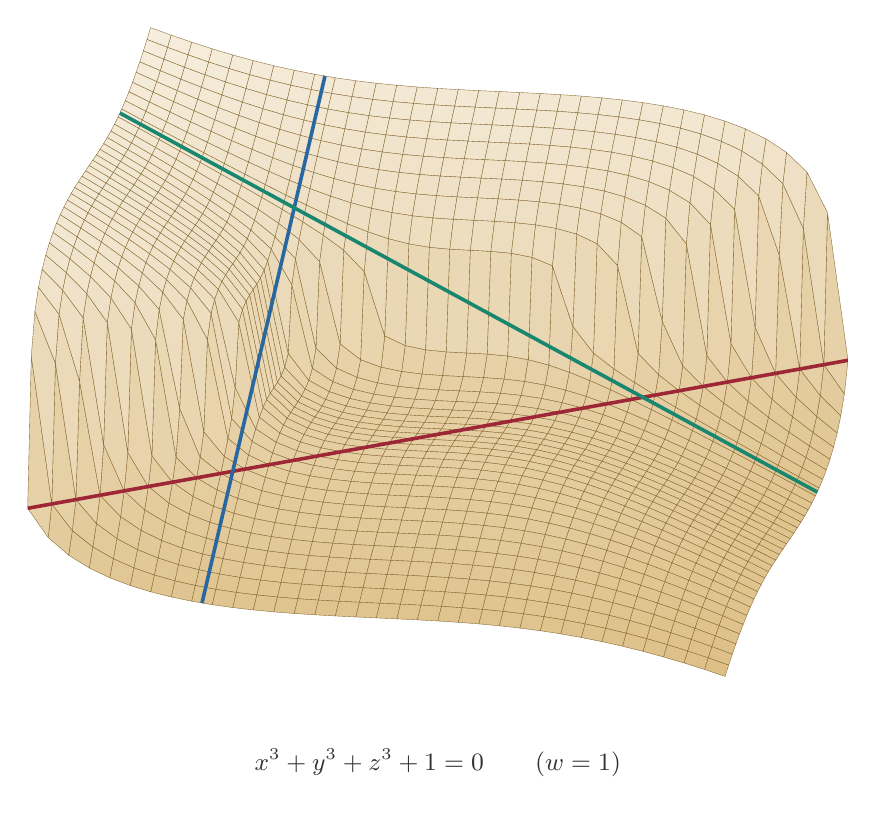
\begin{tikzpicture}
\begin{axis}[
  width=12cm,height=10cm,
  view={100}{22},
  hide axis,
  domain=-2:2,y domain=-2:2,
  samples=35,samples y=35,
  xmin=-2,xmax=2,ymin=-2,ymax=2,zmin=-2.6,zmax=2.6,
  colormap={surface}{color(0cm)=(cubicgold!65);color(1cm)=(cubicgold!18)},
  z buffer=sort,
]
% sign(t)*abs(t)^(1/3) is the REAL cube root of t.
\addplot3[surf,shader=faceted,faceted color=cubicgold!65!black,line width=0.13pt]
  {-sign(1+x^3+y^3)*abs(1+x^3+y^3)^(1/3)};
% The three real lines (i=j=0 in the families below).
\addplot3[lineA,line width=1.3pt,samples=2,samples y=1,domain=-2:2]
  (x,-x,-1) node[pos=.94,above right,font=\small] {};
\addplot3[lineB,line width=1.3pt,samples=2,samples y=1,domain=-2:2]
  (x,-1,-x) node[pos=.96,below left,font=\small] {};
\addplot3[lineC,line width=1.3pt,samples=2,samples y=1,domain=-2:2]
  (-1,x,-x) node[pos=.96,below right,font=\small] {};
\end{axis}
% A small orientation guide, separate from the surface.

\node (equation) [below=8mm,font=\small,text=black!80]
  at (current bounding box.south)
  {$x^3+y^3+z^3+1=0\qquad(w=1)$};
\end{tikzpicture}
\end{lrbox}
\begin{tikzcd}[ampersand replacement=\&,cells={nodes={inner sep=0pt}}]
  \usebox{\surfaceplot}
\end{tikzcd}
\end{document}